\documentclass[a4paper]{article}

\usepackage[english]{babel}
\usepackage{amsmath}
\usepackage{graphicx}
%\usepackage{algorithm}
%\usepackage{algorithmic}
%\usepackage{algpseudocode}
\usepackage{url}


\title{Omega3P Integration Progress Report}

\author{Cameron W. Smith, Gerrett Diamond}

\date{\today}

\begin{document}
\maketitle

\section{In-memory Integration}

Parallel simulations on massively parallel systems are most effective when data
movement is minimized.
Data movement costs increase with the depth of the memory hierarchy; a design
trade-off for increased capacity.
For example, the highest level on-node storage in the IBM BlueGene/Q A2
processor~\cite{haring2012ibm} is the per-core 16KiB L1 cache (excluding
registers) and has a peak bandwidth of 819 GiB/s.
The lowest level on-node storage, 16GiB of DDR3 main memory, provides a million
times more capacity at the cost of 19 times less bandwidth,
43GiB/s~\cite{lo2014roofline}.
One level further down the hierarchy is the parallel filesystem
~\footnote{We assume, for the sake of simplicity, that the main memory of other nodes is not
available.
In practice, most applications do not not use all the on-node memory and some
checkpoint-restart methods take advantage of this for increased performance
~\cite{rma-fault-tolerance-2014,isaila2014making,compression-cr-2012}.
}.
At this level the bandwidth and capacity relationship is less clear as the
filesystem is a shared resource.
Table~\ref{tbl:systems} lists the per-node peak main memory and filesystem
bandwidth across four generations of Argonne National Laboratory leadership
class systems: BlueGene/L~\cite{yu2006high,adiga2002overview}, Intrepid
BlueGene/P~\cite{lang2009performance,alam2008early}, Mira
BlueGene/Q~\cite{haring2012ibm,bui2014scalable}, and 2018's
Aurora~\cite{aurorafacts}.
Based on these peak values the bandwidth gap between main memory and the
filesystem is at least three orders of magnitude.
Software must leverage the cache and main memory bandwidth performance advantage
during as many operations as possible to maximize performance.

\begin{table}[h]
\centering
\caption{Per-node main memory and filesystem peak bandwidth over four
  generations of Argonne National Laboratory systems.
  The values in parentheses indicate the increase relative to
  the previous generation system.}
\label{tbl:systems}
\begin{tabular}{l|cc}
        & Memory BW & Filesystem BW \\
        & (GiB/s)    & (GiB/s)    \\
 \hline
 BG/L   & 5.6       & 0.0039         \\
 BG/P   & 14 (2.4x) & 0.0014 (0.36x)   \\
 BG/Q   & 43 (3.1x) & 0.0049 (3.5x) \\
 Aurora & 600 (14x) & 0.020 (4.1x)
\end{tabular}
\end{table}

Approaches for high performing and scalable component interactions avoid
file-based I/O through in-memory data streams and component functional
interfaces.
The ADIOS tools provide an alternative mechanism for the in-memory coupling of
executables~\cite{bennett2012combining,zhang2012enabling}; our work here focuses
on the interaction of libraries operating within the same process.
Components that support a common file format can use our data stream approach
with minimal software changes to exchange data via memory buffers instead of files.
This approach is also a logical choice for legacy analysis codes that do not
provide functional interfaces to access or create their input and output data
structures.

Components with functional interfaces that encapsulate creation, deletion, and
access to underlying data structures support in-memory interactions.
The level of interface granularity selected for defining interactions has a
proportional impact on flexibility and development costs.
At a very fine level a developer may implement all mesh entity query functions such
that components can share the same mesh structure; trading increased development
costs for lower runtime memory usage.
An excellent example of this is the use of octree structures in the
development of parallel adaptive analyses~\cite{BursteddeWilcoxGhattas11}.
At a coarser level a developer may simply create another mesh
representation through use of interfaces encapsulating mesh construction;
trading higher runtime memory usage for lower development costs.
For example, an existing solver component can embed low level
calls to mesh-entity iterators~\cite{Ollivier10}.
Although this method will allow for in-memory integration, it suffers from the
same disadvantages as a tightly coupled approach in that a significant amount of
time and effort will be required for code modification and verification.
A generalization of this coarser level approach defines common sets of
interfaces through which all components interact.
For example, in the rotorcraft aerodynamics community the HELIOS platform
provides a set of analysis, meshing, adaptation, and load balancing components
via the Python-based Software Integration Framework~\cite{sankaran2010application}.

Our implementation of in-memory integration for PUMI and Omega3p uses
mesh query and construction APIs for mesh and field conversion combined with
fine-level APIs for querying higher-order geometric data for element
integrals.
The mesh conversion approach trades code simplicity for increased peak memory usage.
During PUMI adaptation and load balancing only the PUMI mesh is stored.
After conversion though, we store both the PUMI mesh and the Omega3P
DistMesh.
Mesh conversion alone is not sufficient to integrate over elements near the
geometric boundary.
We support these integrals by implementing Omega3P geometric queries with PUMI
APIs that can interrogate parametric model information provided by CAD
kernels.

\section{Load Balancing}

Omega3P solving step relies on both on part mesh entities as well as a layer of 
ghosted elements along each part boundary. Figure \ref{fig:ghost3} shows an 
example of a mesh with three layers of ghosting. In order to reach maximum efficiency
for ghost based codes partitioning much target minimizing the sum of the 
weights of elements plus the sum of the weights of the ghost elements. 

\begin{figure}[ht]
\centering
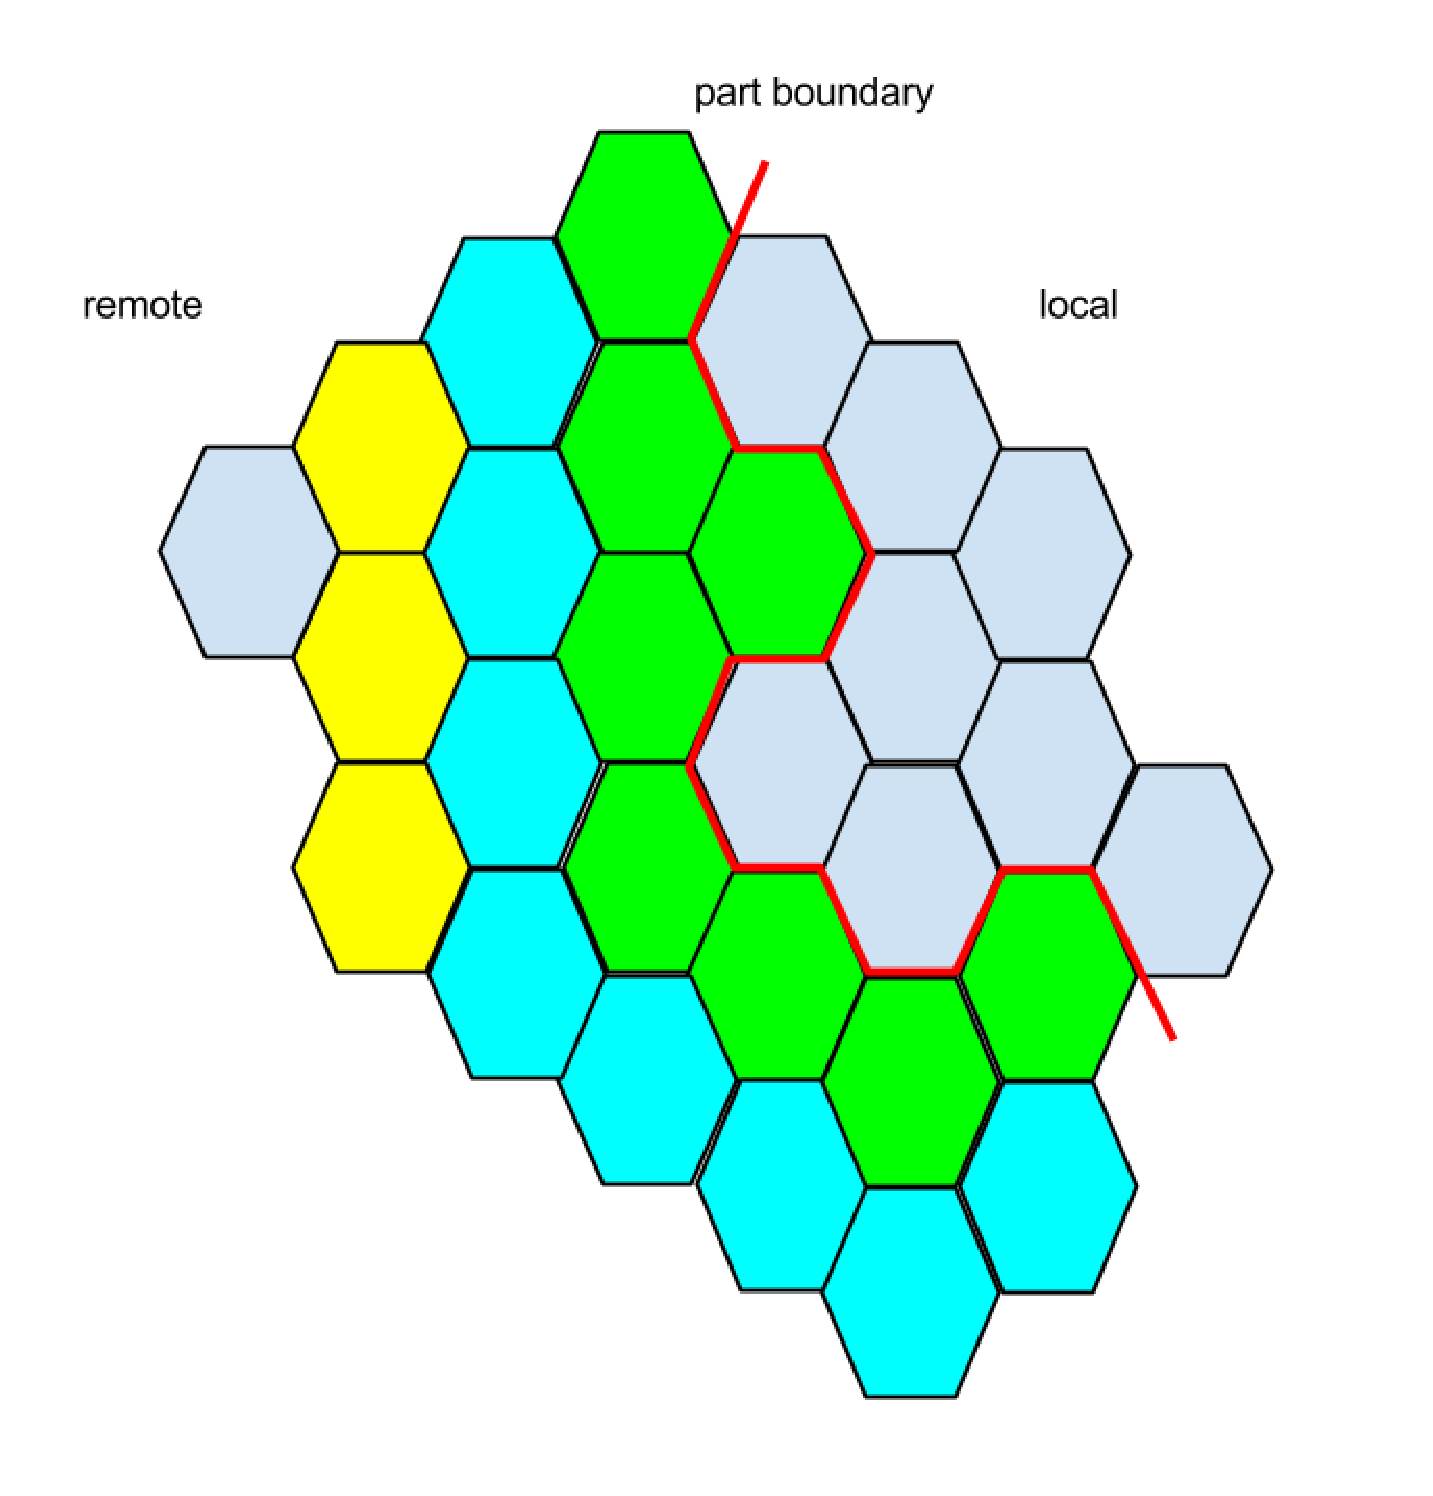
\includegraphics[width=0.4\textwidth]{ghostingExample.eps} 
\caption{\label{fig:ghost3} Three layers of elements ghosted from the remote part to the local part.  The first layer is colored green, the second blue, and the third yellow.}
\end{figure}

\noindent Our strategy for partitioning and load balancing is started with a 
uniformly-weighted 
partition of the mesh from 1 part to $N$ parts followed by ghost-aware diffusive load 
balancing using ParMA~\cite{SmithParma2015} to get a final mesh that is well balanced 
in terms of on-part elements and ghosted elements along the part's boundary. We 
currently utilize ParMA's partition improvement procedures that account for the 
ghosted layers using a combination of existing element selection criteria and an 
extended 'weight' tracking mechanism.  The weight tracking extension relies on the 
exact knowledge of the change to the ghosted elements as elements on a heavy part 
are selected for migration to a light part. The current implementation of these 
procedures assumes vertex-based ghosting while Omega3P ghosting is element-based. 
To accurately accommodate for Omega3P's ghosting we will be extending ParMA's 
ghosting to be able to balance based on element-based ghosting. To further improve 
the efficiency of the load balancing we may explore better partitionings 
that are ghost-aware so that ParMA is given a better initial partitioning such that it 
can find a better partitioning faster.

\section{Status}
In its current state our implementation includes loading the mesh into PUMI/APF, partitioning/load balancing of the PUMI/APF mesh and transfer from PUMI/APF to Omega3P's mesh data structure. The conversion process works for both straight-sided elements and second order curved geometry.

\section{Results}

We compared the runtime and memory usage of Omega3P versus Omega3P+PUMI on
up to 128 cores of the NERSC Cori Phase I system
Runtime data is listed in Table~\ref{tbl:time}.
Peak memory usage data gathered from runs is listed in Table~\ref{tbl:memusage}.

\begin{table}[h]
\centering
  \caption{Runtime of Omega3P verus Omega3P+PUMI.}
\label{tbl:time}
\begin{tabular}{l|cc}
        & Memory BW & Filesystem BW \\
        & (GiB/s)    & (GiB/s)    \\
 \hline
 BG/L   & 5.6       & 0.0039         \\
 BG/P   & 14 (2.4x) & 0.0014 (0.36x)
\end{tabular}
\end{table}


\begin{table}[h]
\centering
  \caption{Peak memory usage of Omega3P verus Omega3P+PUMI.}
\label{tbl:memusage}
\begin{tabular}{l|cc}
        & Memory BW & Filesystem BW \\
        & (GiB/s)    & (GiB/s)    \\
 \hline
 BG/L   & 5.6       & 0.0039         \\
 BG/P   & 14 (2.4x) & 0.0014 (0.36x)
\end{tabular}
\end{table}



\newpage
\bibliographystyle{plain}
\bibliography{scorec-refs/partition,scorec-refs/meshdb,scorec-refs/hardware,scorec-refs/io,scorec-refs/frameworks,scorec-refs/cr.bib}


\end{document}


